\section{Random Fields and Spin Glasses}
\subsection{Setting up the Random Field Problem}
We consider the Hamiltonian:
\begin{equation}
    H = \int d^dx \left(\frac{1}{2}\kappa (\nabla s)^2 + \frac{1}{2}ts^2 + \frac{1}{4}us^4 - \v{h}(x)\cdot \v{s}\right)
\end{equation}
where:
\begin{equation}
    \overline{h_i(\v{x})h_j(\v{x}')} = \delta_{ij}\Delta \delta (\v{x} - \v{x}')
\end{equation}
i.e. we have a random uncorrelated field. Although it is written down as a magnet, it is a kind of model that emerges very frequently in random media. For example, an elastic medium sitting on a surface which is random, causing the elastic to stretch in some ways.

\begin{center}
    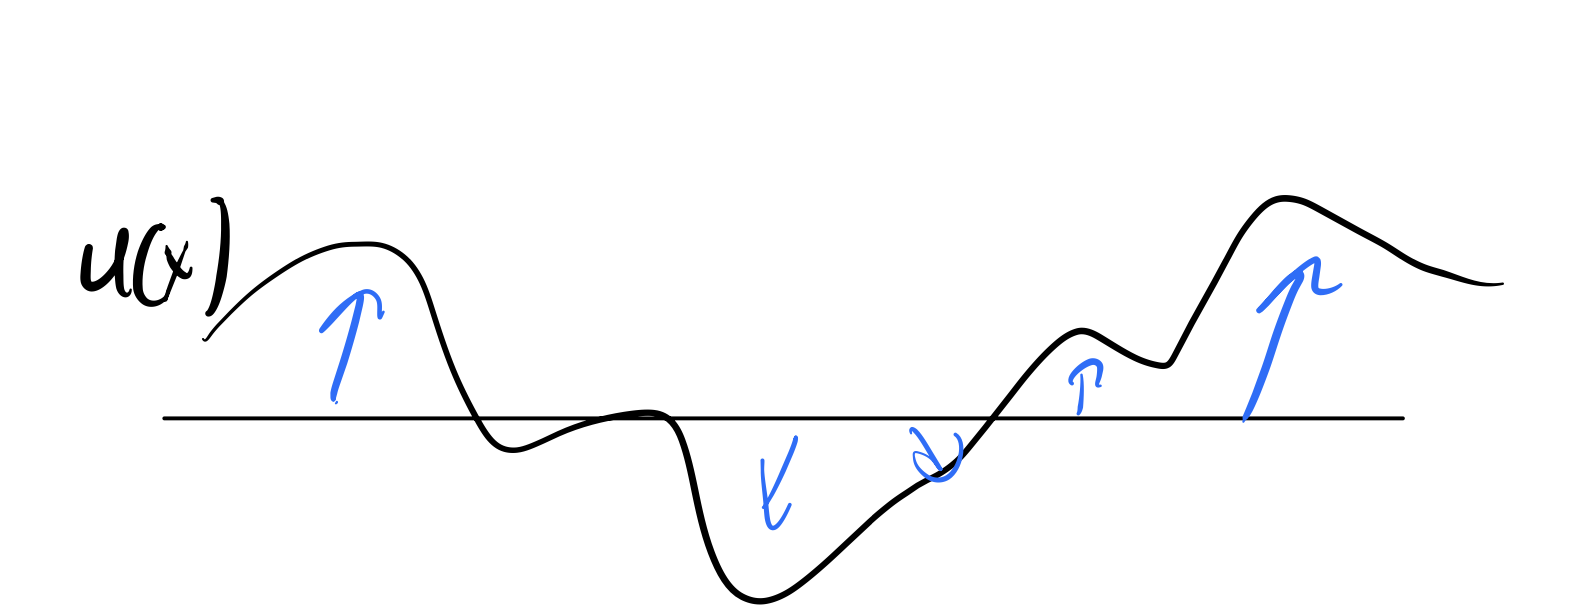
\includegraphics[scale=0.35]{Lectures/Figures/lec13-randomelastic.png}
\end{center}

Consider random fields $h_i$. If we RMS average over a length scale $L$:
\begin{equation}
    \sqrt{\sum_{i=1}^L h_i^2} = h_0\sqrt{cL^d}
\end{equation}
where $h_0$ is a strength and $c$ a concentration. This $\sim \sqrt{N}$ comes from a random walk.

If we average and get some nonzero up spin, and average in a neighbouring region and get a nonzero down spin, then we get an energy penalty. We have a gain of the form $h_0 L^{d/2}$ (from the spins within a domain aligning with the local field, from the $\v{h}_i \cdot \v{S}_i$ term) and a loss of the form $JL^{d-1}$ (coming from the penalty of interacting neighbouring domains, the $\v{S}_i \cdot \v{S}_{i+1}$ term). When do each of the terms win out? When $\frac{d}{2} > d-1$, i.e. when $d < 2$, the energy gain wins.

\subsection{Solving the model}
To attack this model, we consider the replica trick:
\begin{equation}
    \overline{Z^n} = \int \mathcal{D}h(x) P(h(x)) \prod_{a=1}^n \int dS_a e^{-\beta H[S_a, h]}
\end{equation}
We take the distribution of the fields to be Gaussian:
\begin{equation}
    P(h) \sim e^{-\frac{h^2}{\Delta}}
\end{equation}
This allows us to write:
\begin{equation}
    \overline{Z^n} = \prod_a \int dS_a e^{-\beta H_{\text{eff}}[S_a, S_b]}
\end{equation}
with:
\begin{equation}
    H_{\text{eff}} = \int d^dx\left[\sum_{a=1}^n \frac{1}{2}\kappa (\nabla s_a)^2 + \frac{1}{2}ts_a^2 + + \frac{1}{4}us_a^4\right] - \frac{1}{2}\beta \sum_{a, b}\Delta \v{s}_a \cdot \v{s}_b
\end{equation}
(Rio note: This expression doesn't looks like it makes sense with the sum over $a, b$s, but so be it.) Going to momentum space:
\begin{equation}
    H_{\text{eff}} = \frac{1}{2}\int \frac{d^dk}{(2\pi)^d}\left(\sum_{a, b}(\kappa k^2 +t)\delta_{ab}  - \beta \Delta J_{ab}\right)s_a(k)s_b(-k) + \frac{u}{4}s^4
\end{equation}
with $J_{ab}$ just a matrix of 1s everywhere. If we had no fourth order term, we can view this as a Green's function:
\begin{equation}
    \avg{s^i_a(k)s^j_b(k')} = G^0_{ab}\delta(k + k')
\end{equation}
with:
\begin{equation}
    G^0_{ab}(k) = \delta_{ij}\left[\frac{T}{\kappa k^2 + t}\delta_{ab} + \frac{\Delta}{(\kappa k^2 + t)^2}J_{ab}\right]
\end{equation}

If we study the scaling:
\begin{equation}
    \kappa \to \kappa b^{d-2+2\zeta}
\end{equation}
\begin{equation}
    t \to tb^{d+2\zeta}
\end{equation}
\begin{equation}
    u \to ub^{d+4\zeta}
\end{equation}
\begin{equation}
    \frac{\Delta}{T} \to b^{d+2\zeta}\frac{\Delta}{T} = b^2\Delta
\end{equation}
with $\zeta = \frac{2-d}{2}$ where we recall that we have the RG scaling parameters from $s \to b^\zeta s$. We see that $\Delta$ has a positive eigenvalue and is therefore a relevant exponent. There is a new relevant field in the vicinity of the fixed point, and we flow away.

\begin{center}
    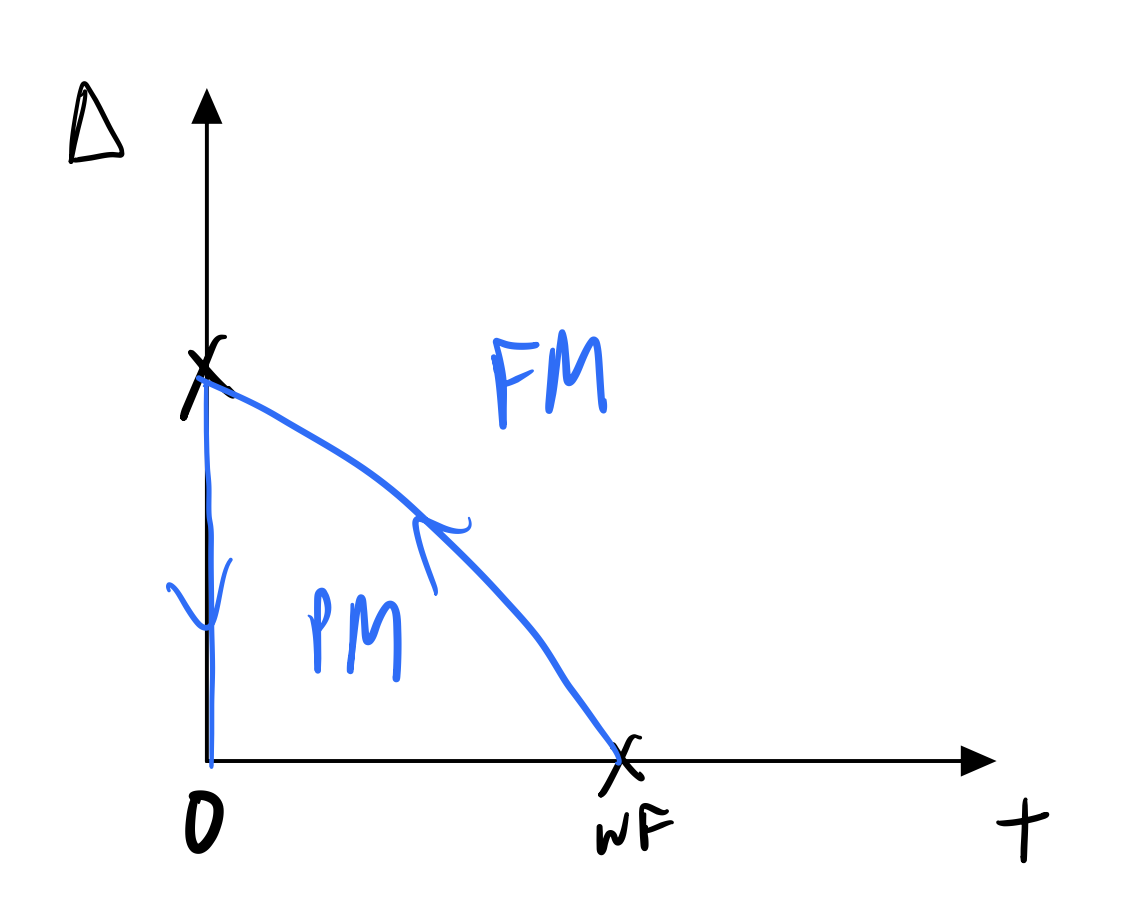
\includegraphics[scale=0.35]{Lectures/Figures/lec13-randomrgflow.png}
\end{center}

The fixed point Hamiltonian is:
\begin{equation}
    H^* = \int d^dx \left[\frac{1}{2}\kappa(\nabla s)^2\right]
\end{equation}
If we ask what is $\avg{\delta s^2}_{\text{thermal}}$, this is something we've seen before:
\begin{equation}
    \avg{\delta s^2}_{\text{thermal}} = \int_{1/L}^\infty \frac{d^dk}{(2\pi)^d}\frac{T}{\kappa k^2}
\end{equation}
Now we want to ask how this scales depending on the lower momentum cutoff $L$. By a scaling argument, we see:
\begin{equation}
    \avg{\delta s^2}_{\text{thermal}} \sim \frac{T}{\kappa}L^{2-d}
\end{equation}
If I look at the random field Hamiltonian we have the $\frac{\Delta}{(\kappa k^2 + t)^2}$ term. Then we have:
\begin{equation}
    \avg{\delta s^2}_{RF} \sim \int_{1/L}^\infty \frac{d^dk}{(2\pi)^d}\frac{\Delta}{\kappa^2k^4} = \frac{\Delta}{\kappa^2}L^{4-d}
\end{equation}
We then get the length scale over which one term wins:
\begin{equation}
    \xi = \left(\frac{\kappa}{\Delta}\right)^{\frac{1}{4-d}}
\end{equation}
In $D > 4$, this is minimized as $L \to \infty$, as $D < 4$ the length scale is finite.

Remark: Formal theory arguments gave $D = 3$ for a long time, in contrast with the quick argument we have here. It turns out the reason is that high-dimensional domain walls are hard. This is a reminder that back-of-the-envelope intuition is better than formal theory.

If we have an EOM:
\begin{equation}
    \nabla^2 \psi + t\psi = h
\end{equation}
with $h$ a source, then:
\begin{equation}
    \psi_k = \frac{h_k}{k^2 + t}
\end{equation}
and so:
\begin{equation}
    \avg{\psi_k\psi_{k}} = \frac{\avg{h_k}}{(k^2 + t)^2}
\end{equation}
We'll stop here on random fields, but this is a rather generic problem. There are many scenarios where we get this type of equation of motion.

\subsection{Ergodicity}
Every system we've thought about so far has been ergodic. Namely, $Z$ has been the average over all possible configuration, and the system is assumed to explore all of them. It turns out that the heart of exploring glasses is the breaking of this ergodicity.

Fundamentally, what this means is that if we go down to low temperature, the system gets trapped in a region of phase space, and cannot explore the rest of it. Notably, if we heat up the glass and cool it back down, it will go to a different region.

We define broken ergodicity as:
\begin{equation}
    \avg{\cdot} = \sum_\alpha \omega_\alpha \avg{\cdot}_\alpha
\end{equation}
with $\alpha$ a pure state.
For example in the FM Ising model:
\begin{equation}
    \avg{\sigma} = \frac{1}{2}\avg{\sigma}_+\frac{1}{2}\avg{\sigma}_- = 0
\end{equation}
There is a tendency for pure states to cluster; for example:
\begin{equation}
    \avg{\sigma_i\sigma_j} \to \avg{\sigma_i}\avg{\sigma_j} \text{ for } \abs{i - j} \to \infty
\end{equation}
which means that the connected correlation function goes to zero.

Suppose we have some internal state $\alpha$ and a state $\beta$ outside.

\begin{center}
    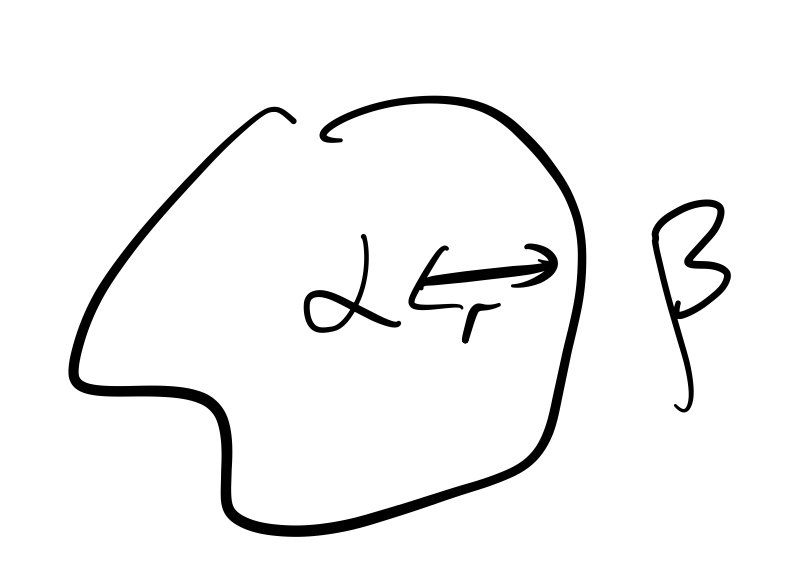
\includegraphics[scale=0.3]{Lectures/Figures/lec13-statesize.png}
\end{center}

We can define a length scale $r$ of the $\alpha$ droplet, and compute the free energy difference of the two terms:
\begin{equation}
    \Delta F = \sigma r^{d-1} - (\delta f)r^d
\end{equation}
where $\delta f$ is $F_\alpha - F_\beta$. This defines a $r_{max}$ where the free energy difference is maximized:
\begin{equation}
    r_{\text{max}} = \frac{\sigma(d-1)}{d\delta f}
\end{equation}
Looking at the maximum difference in the free energy (the barrier):
\begin{equation}
    \Delta F_{\text{max}} = \sigma\left(\frac{\sigma}{\delta f}\right)^{d-1}\left(\left(\frac{d-1}{d}\right)^{d-1} - \left(\frac{d-1}{d}\right)^{d}\right)
\end{equation}
Either $d \to \infty$ or $\delta f \to 0$ means we have large barriers between states. The latter case is find because we have two states with the same energy. $d \to \infty$ is also interesting as then the large dimension provides a big penalty/barrier.

\begin{center}
    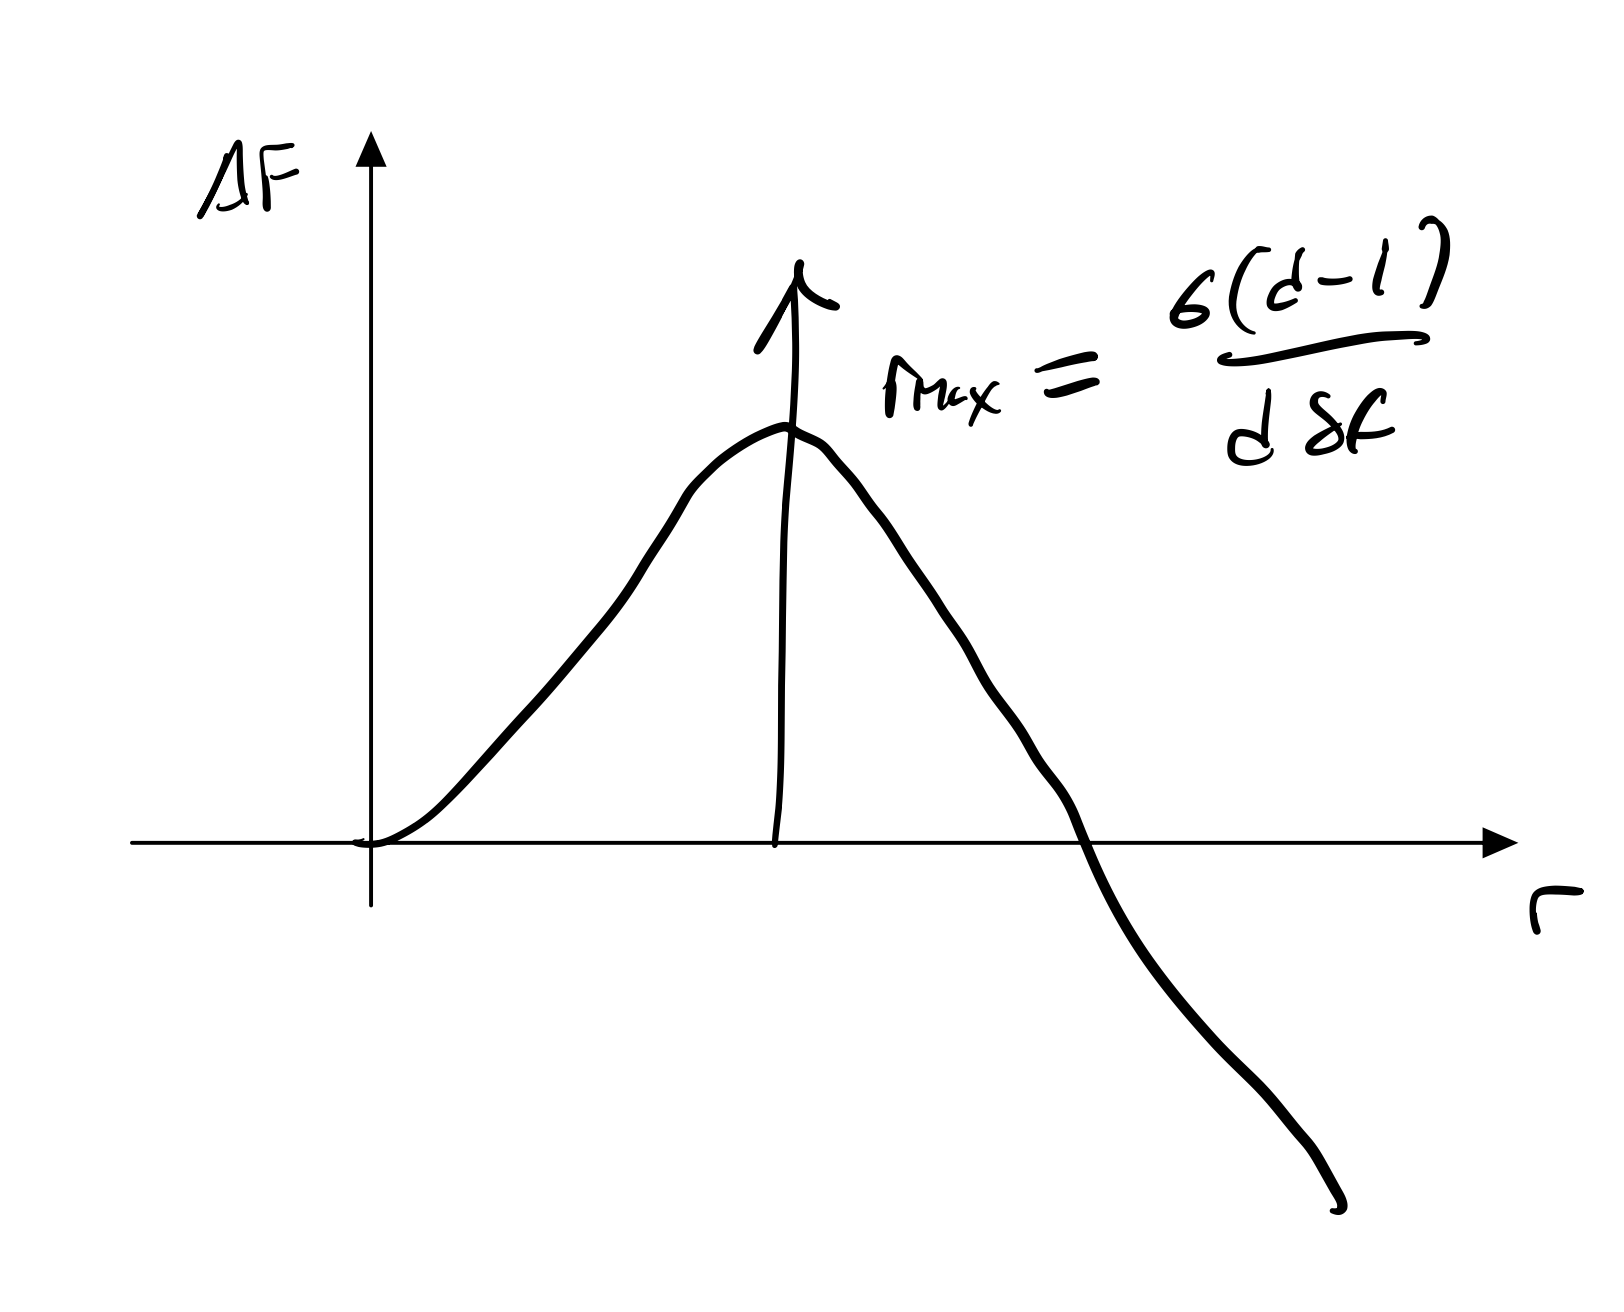
\includegraphics[scale=0.35]{Lectures/Figures/lec13-freeenergybarrier.png}
\end{center}

Next day, we look at a infinite range glass model, which is exactly solvable. At infinite temperature, despite not having any order, it has many ground states whose energies are the same, related by hierarchies.

\subsection{Order parameters}
Previously, we looked at the magnetization:
\begin{equation}
    m = \frac{1}{N}\sum_{i=1}^N \avg{\sigma_i}
\end{equation}
now we are interested in states that freeze, but do not order. This gives rise to an order parameter proposed by Edwards and Anderson, wich looks like:
\begin{equation}
    q_{EA} = \frac{1}{N}\sum_{i=1}^N \avg{\sigma_i}^2
\end{equation}
where we look at the square of the average. The spin could in principle point in any direction, which I don't care about; I care about whether the thermal average could persist forever. This is something that one in principle could atempt to measure, and would distinguish between a paramagnetic state, and a frozen but disordered state. We can generealize this to overlaps:
\begin{equation}
    q_{\sigma\tau} = \frac{1}{N}\sum_{i=1}^N \sigma_i \tau_i
\end{equation}
which taking averages:
\begin{equation}
    Q_{\alpha\beta} = \frac{1}{N}\sum_{i=1}^N \avg{\sigma_i}_{\alpha}\avg{\tau_i}_{\beta}
\end{equation}
These overlaps allow us to probe the structure in phase space. In low temperature FM, $Q_{\alpha\alpha} = 1$ while $Q_{\alpha\beta} = 0$. Conversely, for the paramagnetic states everything is zero. More concretely, $q_{++} = q_{--} = m^2$ and $q_{+-} = q_{-+} = -m^2$.